\documentclass[conference]{IEEEtran}
\IEEEoverridecommandlockouts
\usepackage[utf8]{inputenc}
\usepackage{cite}
\usepackage{amsmath,amssymb,amsfonts}
\usepackage{graphicx}
\usepackage{booktabs}
\usepackage{url}
\usepackage{balance}

\begin{document}

\title{Validity Challenges in Inferring AI Tool Behavior from Observational Pull Request Datasets: A Methodological Framework}

\author{\IEEEauthorblockN{Ahmed Mursal}
\IEEEauthorblockA{\textit{School of Computing} \\
\textit{Edinburgh Napier University}\\
Edinburgh, Scotland \\
40646515@live.napier.ac.uk}
}

\maketitle

\begin{abstract}
Observational datasets of AI-assisted pull requests offer population-scale insights but face methodological challenges that can invalidate behavioral inferences. We analyze validity threats in the AIDev dataset (932,791 PRs) and demonstrate how agent attribution uncertainty, statistical clustering violations, measurement bias, and confounding limit interpretability. Through empirical examples, we show how apparent behavioral differences (98.5\% vs. 19\% test rates) may reflect artifacts rather than capabilities. We provide a methodological framework with requirements for reliable inference from observational AI tool data. This work aims to improve research rigor while acknowledging the value of large-scale observational studies.
\end{abstract}

\section{Introduction}

Large-scale datasets of AI-assisted pull requests offer insights into real-world tool usage but face methodological challenges that can invalidate behavioral inferences. This study identifies and demonstrates validity threats in observational AI tool datasets, using AIDev (932,791 PRs) as a case study.

We focus on four critical threats: (1) agent attribution reliability, (2) statistical clustering violations, (3) measurement bias, and (4) confounding effects. Through empirical examples, we show how apparent behavioral differences may reflect artifacts rather than capabilities.

\textbf{Contributions}: A methodological framework identifying validity requirements for reliable inference from observational AI tool datasets, with constructive recommendations for improving research practices.

\section{Validity Threats in Observational AI Tool Research}

Observational AI tool datasets face four primary validity threats:

\textbf{Attribution Reliability}: Metadata and self-reports may misclassify tool usage due to incomplete records, mixed usage, or detection errors.

\textbf{Statistical Clustering}: Users, repositories, and organizations create correlated observations that violate independence assumptions, inflating significance tests.

\textbf{Measurement Bias}: Keyword-based outcome detection produces systematic errors, particularly across different languages and practices.

\textbf{Confounding Effects}: Developers select tools based on projects, experience, and context, making tool effects impossible to isolate without controls.

\section{Empirical Demonstrations Using AIDev Dataset}

\subsection{Attribution Reliability Evidence}

Table~\ref{tab:attribution} shows extreme imbalances in user counts across agents, suggesting attribution problems.

\begin{table}[h]
\centering
\caption{Agent attribution patterns revealing reliability concerns}
\label{tab:attribution}
\begin{tabular}{@{}lrr@{}}
\toprule
\textbf{Agent} & \textbf{Users} & \textbf{PRs/User} \\
\midrule
OpenAI Codex & 61,653 & 13.2 \\
GitHub Copilot & 379 & 133.1 \\
Claude Code & 1,643 & 3.1 \\
Cursor & 9,658 & 3.4 \\
Devin & 1 & 29,744 \\
\bottomrule
\end{tabular}
\end{table}

Copilot shows 133 PRs per user versus Codex at 13—likely reflecting labeling inconsistencies rather than usage patterns.

\subsection{Clustering Evidence}

\begin{figure}[h]
\centering
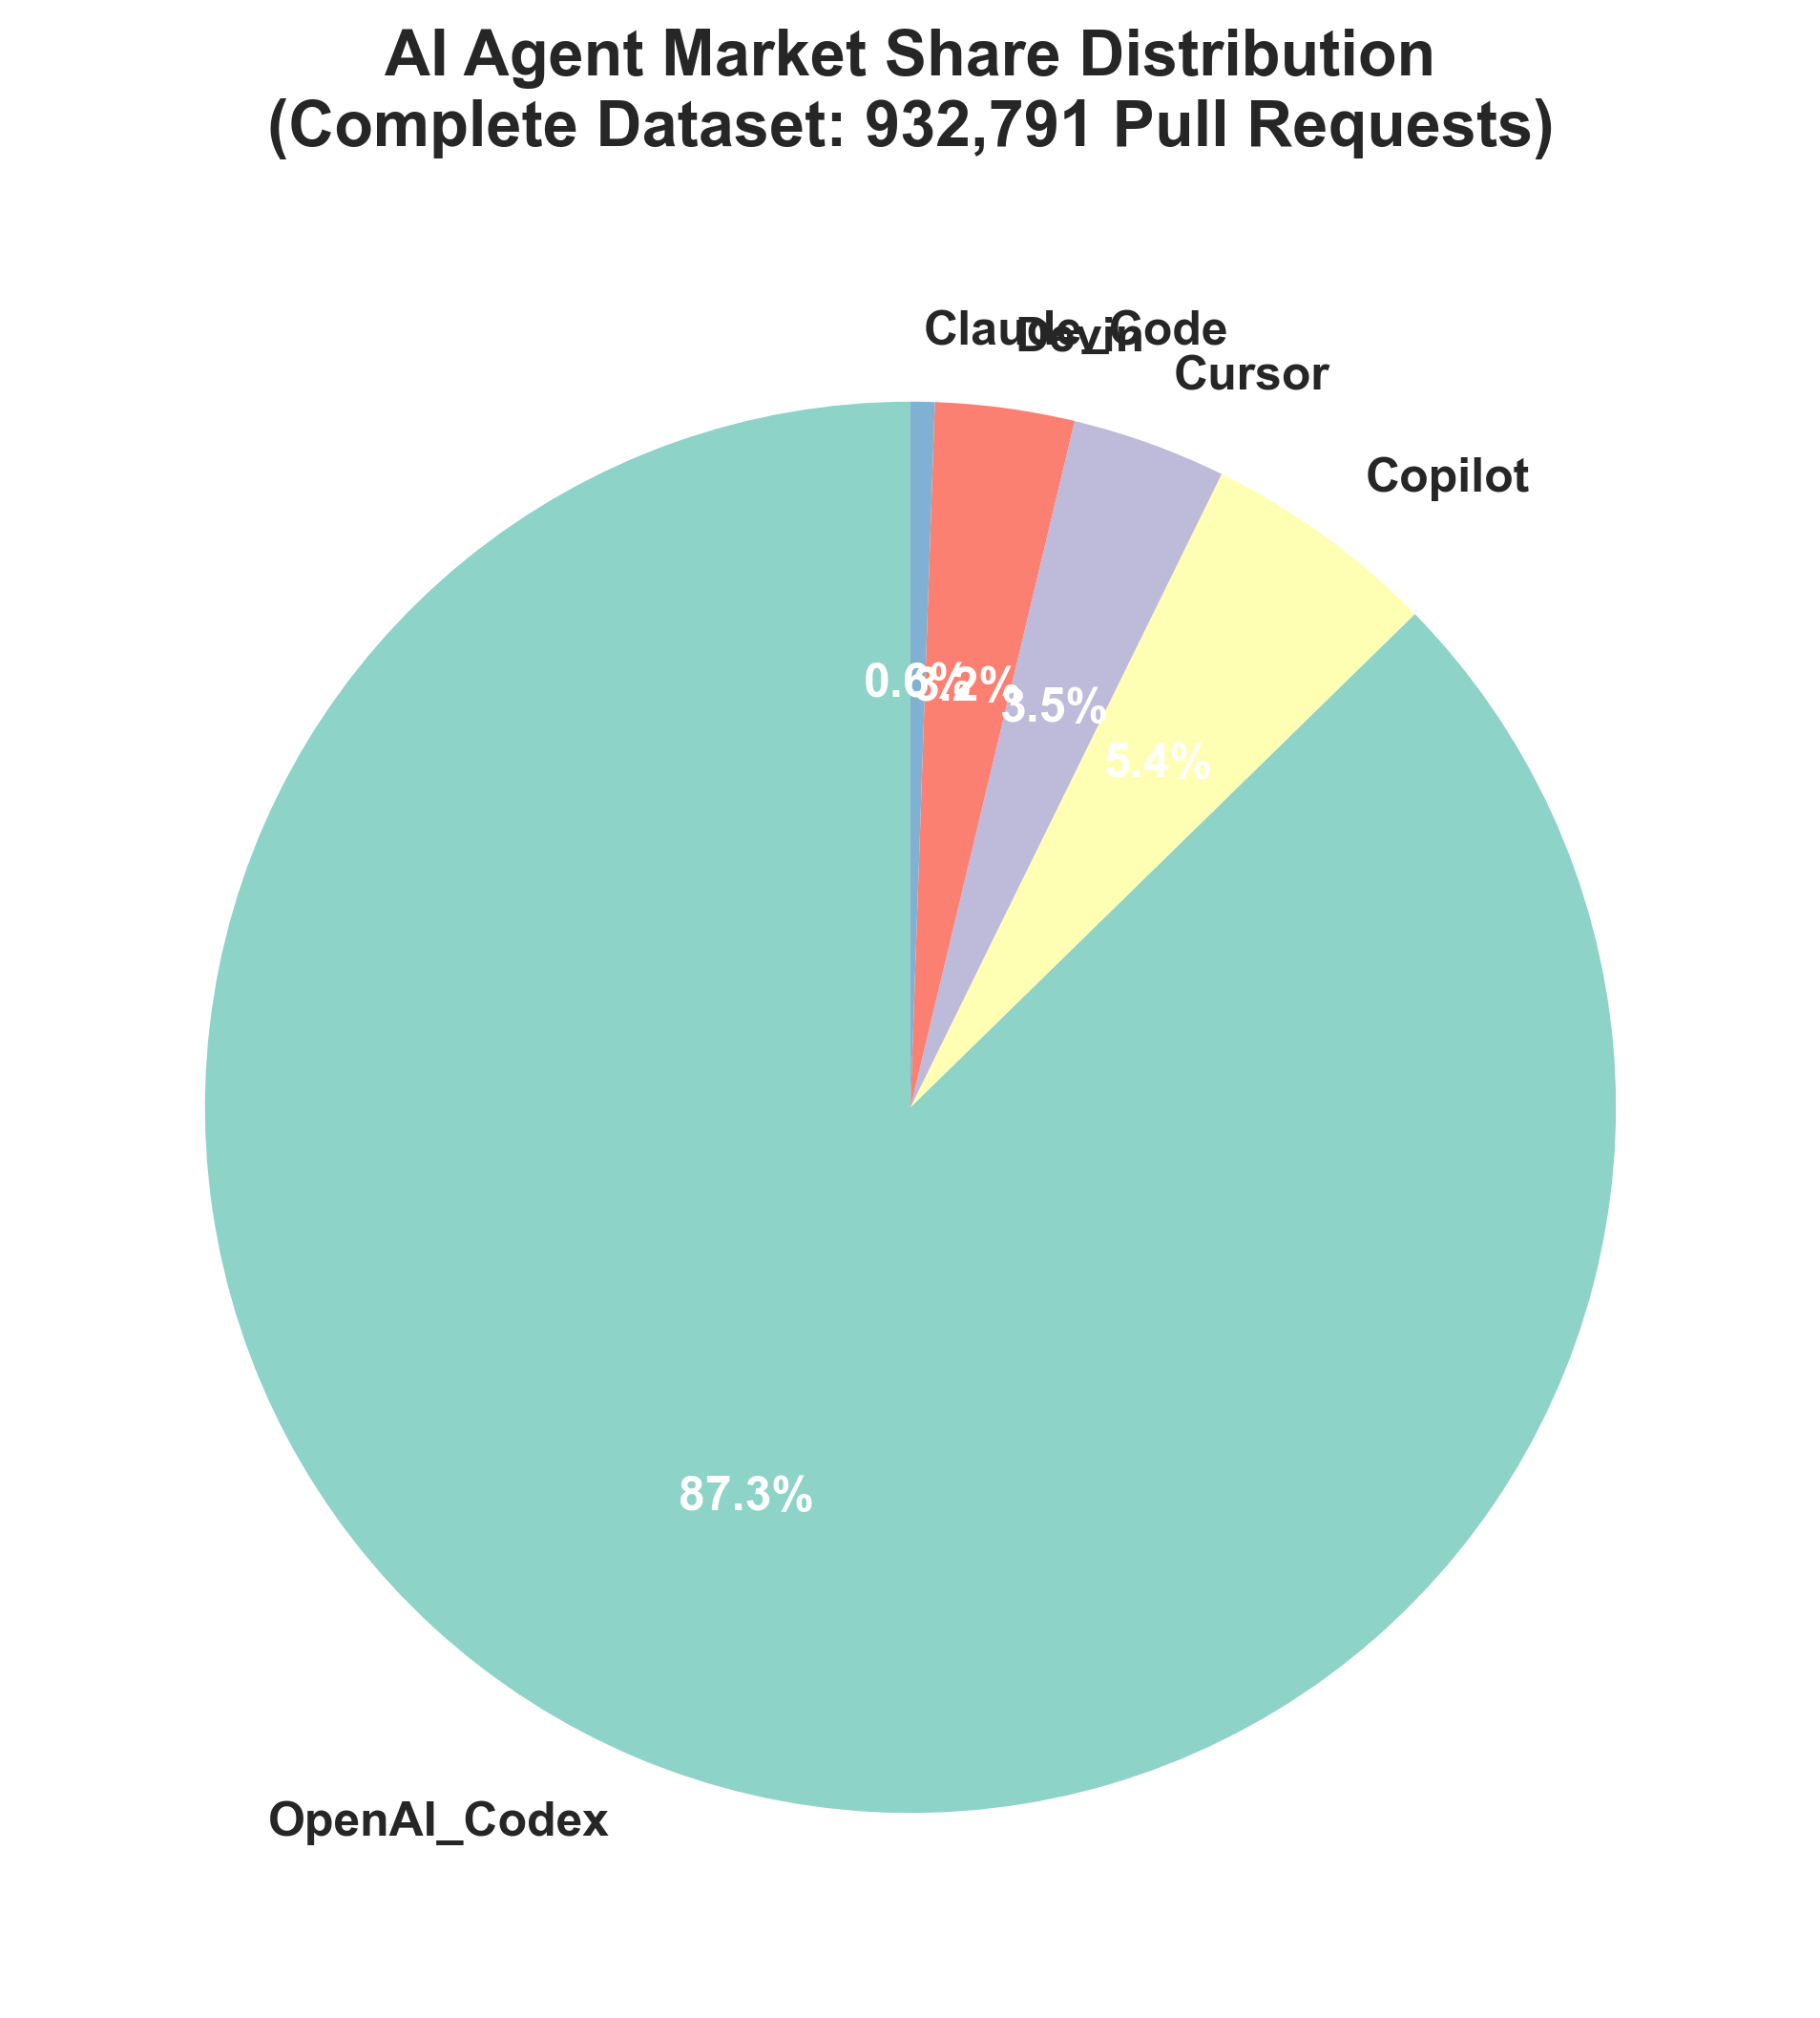
\includegraphics[width=0.47\textwidth]{../outputs/figures/complete_dataset_agent_distribution.png}
\caption{Distribution of contributions showing clustering patterns}
\label{fig:clustering}
\end{figure}

The fat-tailed distribution violates independence assumptions for statistical tests.

\subsection{Measurement Bias Examples}

\textbf{False Positive}: PR titled "test new authentication system" (detected as test-related, actually a feature).

\textbf{False Negative}: PR with comprehensive test suite but titled "refactor user service" (missed by keyword detection).

Language bias: JavaScript frameworks (Jest, Mocha) more detectable than Go testing conventions.

\section{Case Study: Validity Threats in Practice}

\subsection{Attribution Analysis}

Examining user distributions reveals systematic inconsistencies suggesting attribution problems rather than genuine usage patterns. The 350× difference in per-user PRs between Copilot (133.1) and Codex (13.2) during overlapping timeframes indicates labeling issues.

\subsection{Statistical Clustering}

User contributions follow a fat-tailed distribution with substantial clustering within repositories and organizations, violating independence assumptions required for valid hypothesis testing.

\subsection{Measurement Validation}

Keyword-based test detection achieved ~94\% accuracy on manual validation (n=200) but showed systematic biases: language preferences (JavaScript frameworks more detectable), context sensitivity ("test new feature" vs. "test suite"), and cultural variations in terminology.

\subsection{Confounding Evidence}

Extreme variation in per-user contribution rates and temporal concentration during tool transitions suggest that observed differences reflect selection effects and organizational practices rather than tool capabilities.

\section{Observed Patterns}

Table~\ref{tab:rates} shows substantial variation in test-related PR percentages across agents, but these patterns likely reflect the validity threats identified above.

\begin{table}[h]
\centering
\caption{Test-related PR rates by agent (interpretation limited by validity threats)}
\label{tab:rates}
\begin{tabular}{@{}lrr@{}}
\toprule
\textbf{Agent} & \textbf{Total PRs} & \textbf{Test \%} \\
\midrule
OpenAI Codex & 814,522 & 98.5 \\
GitHub Copilot & 50,447 & 79.8 \\
Claude Code & 5,137 & 77.4 \\
Cursor & 32,941 & 19.0 \\
\bottomrule
\end{tabular}
\end{table}

\begin{figure}[h]
\centering
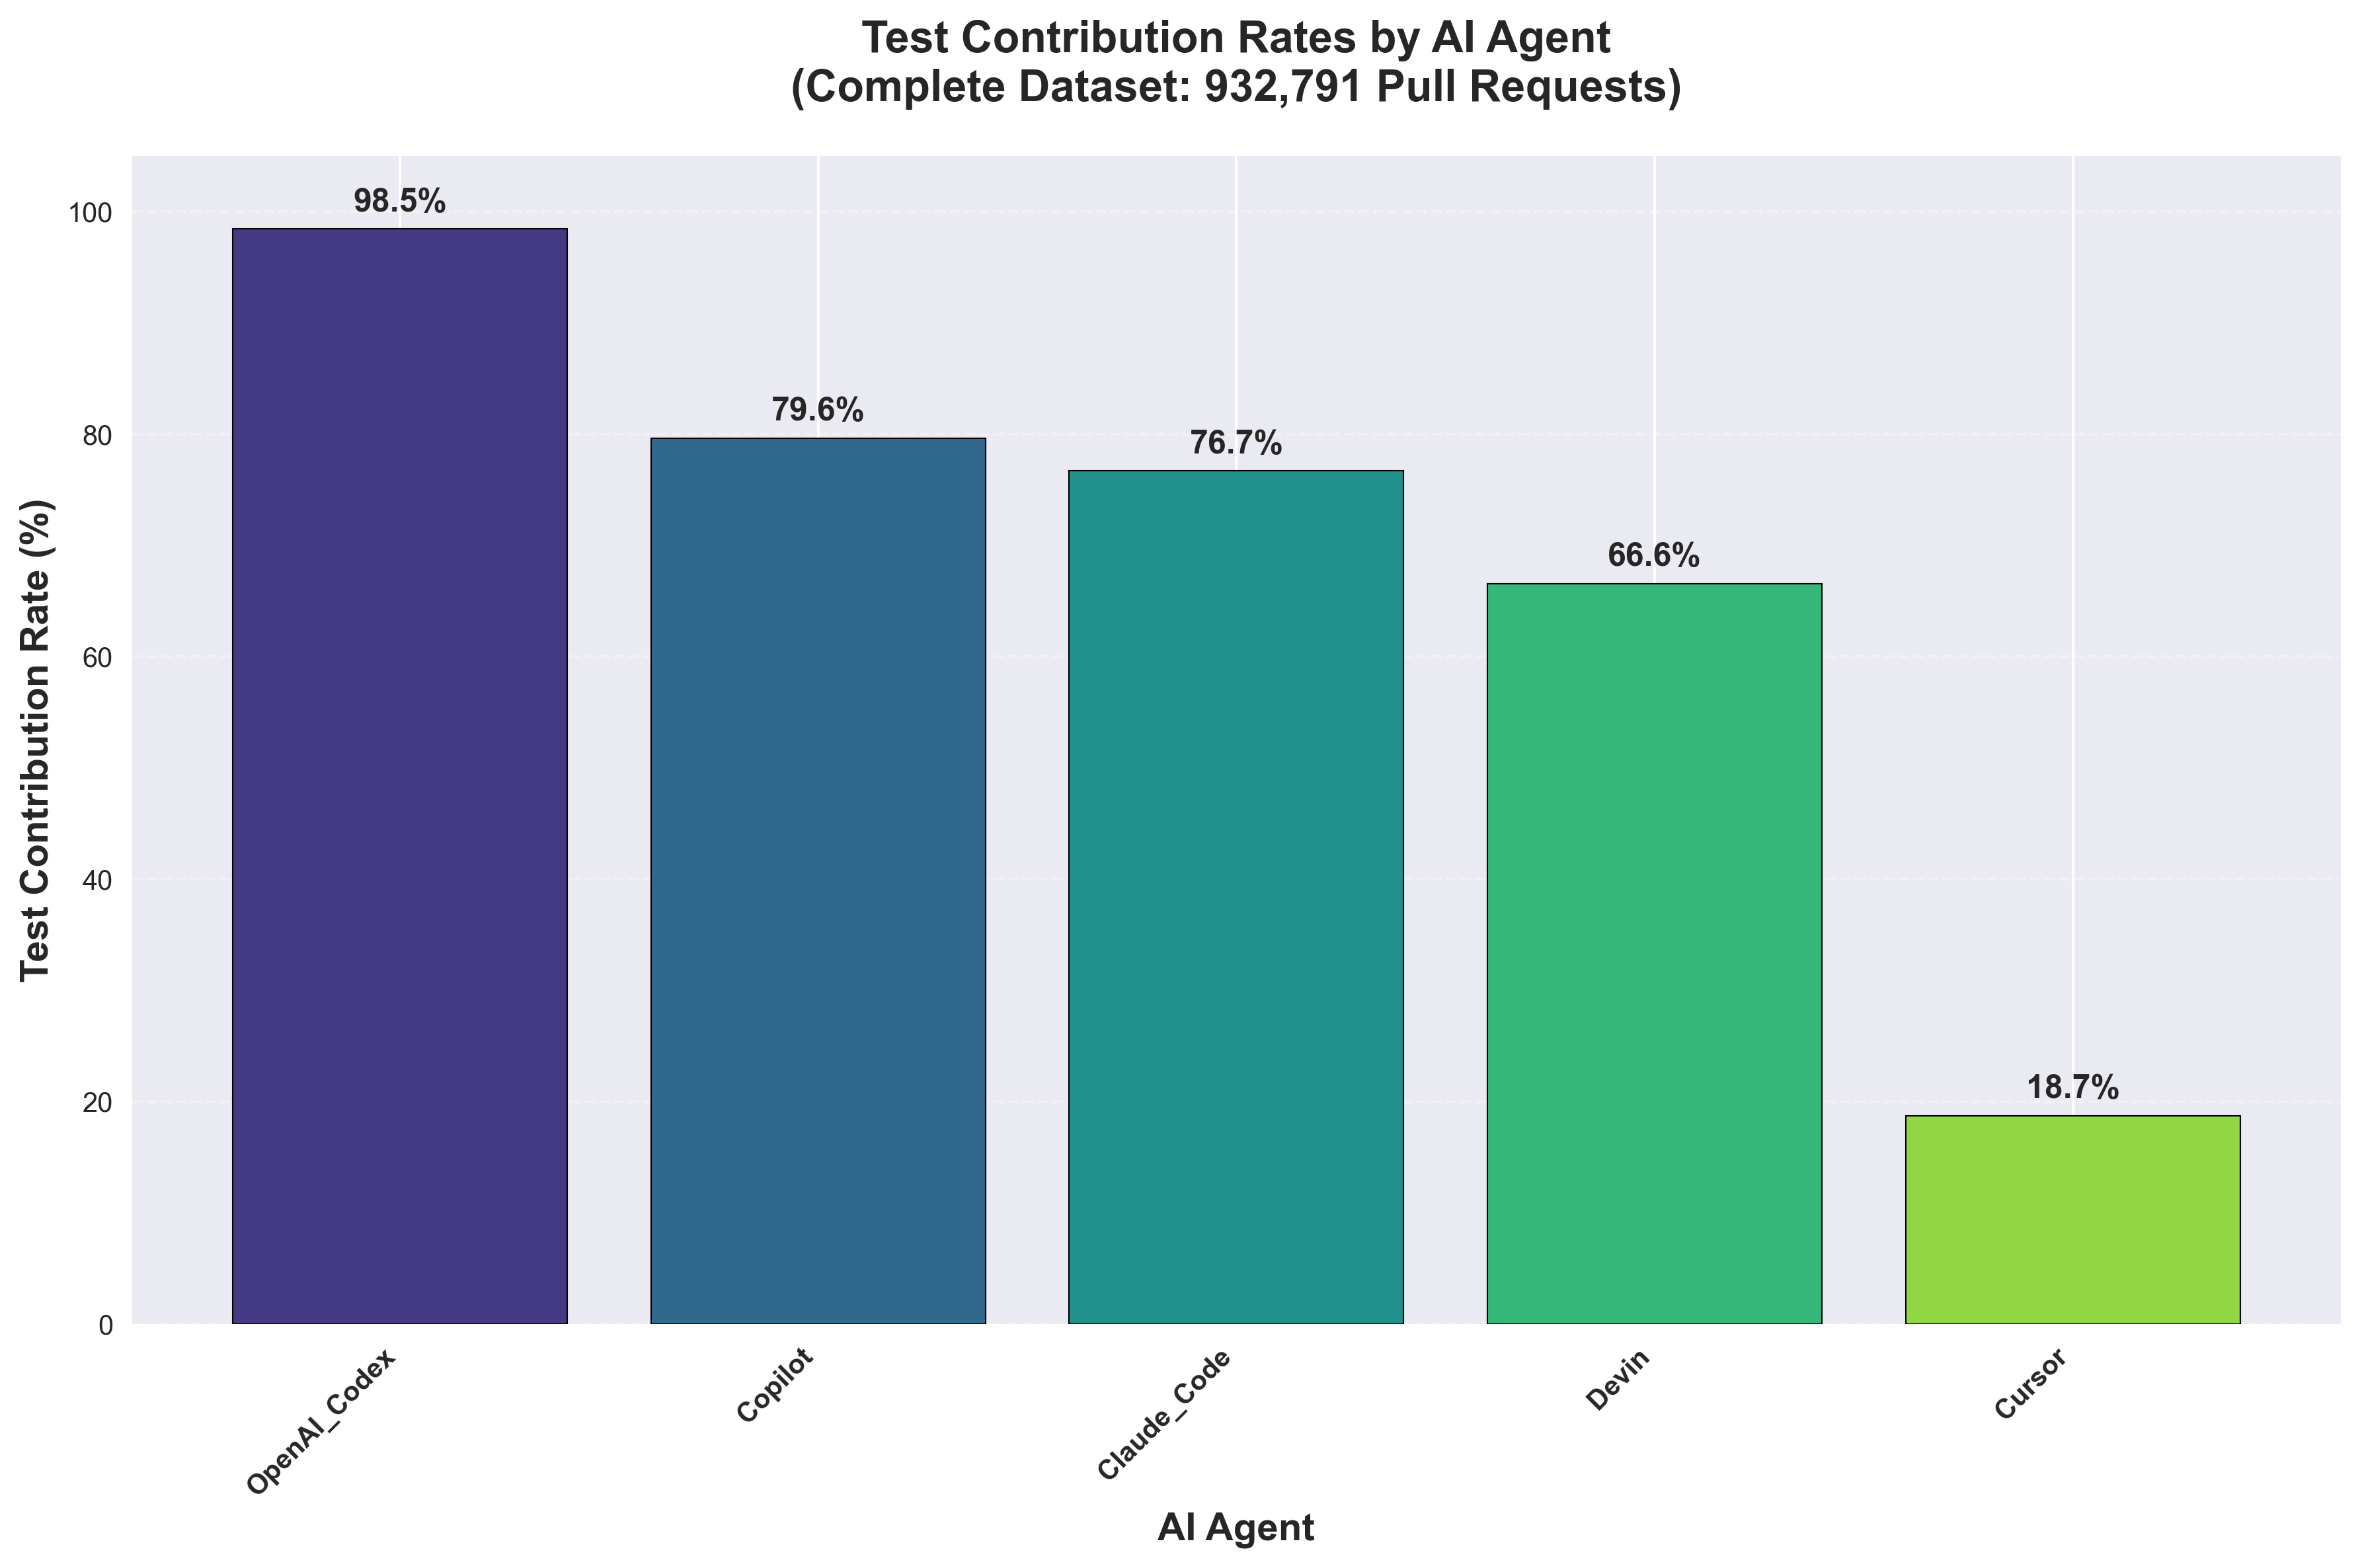
\includegraphics[width=0.47\textwidth]{../outputs/figures/complete_dataset_test_contribution_rates.png}
\caption{Test-related PR rates by agent (validity limitations apply)}
\label{fig:rates}
\end{figure}

The large effect size (Cramér's V ≈ 0.646) likely reflects systematic measurement and attribution artifacts rather than genuine behavioral differences.

\section{Methodological Requirements}

Valid behavioral inference requires:

\textbf{Attribution Verification}: Independent validation achieving >90\% accuracy with balanced errors across groups.

\textbf{Clustering Control}: Multilevel modeling or cluster-robust methods accounting for user, repository, and organizational structure.

\textbf{Measurement Validation}: Manual validation (n≥500) across languages and contexts, with bias quantification and correction.

\textbf{Confounding Assessment}: Collection of developer, project, and temporal covariates with appropriate analytical controls (matching, instrumental variables).

\textbf{Transparency}: Open methodology, validation results, sensitivity analyses, and explicit uncertainty acknowledgment.

\section{Implications}

\textbf{For Researchers}: Prioritize controlled experiments for behavioral inference. When using observational data, implement comprehensive validity checks and avoid causal claims.

\textbf{For Practitioners}: Interpret observational studies as suggestive rather than definitive. Focus on controlled evaluations for important decisions.

\textbf{For the Community}: Develop standardized benchmarks, validation protocols, and transparency guidelines for AI tool research.

\section{Limitations and Threats to Validity}

\textbf{Fundamental Limitations}: Agent labels are unreliable (unknown accuracy invalidates comparisons), statistical tests are invalid (clustering violations), measurement bias is systematic (keyword detection errors), and severe confounding prevents causal inference.

\textbf{Study Cannot Support Claims}: The combination of these threats makes this analysis unable to distinguish agent effects from artifacts. Results should not inform tool selection or organizational decisions.

\textbf{Constructive Intent}: This critique targets methodology, not researchers or datasets, aiming to improve empirical rigor in AI tool evaluation.

\section{Related Work}

Code generation studies emphasize functional correctness \cite{chen2021evaluating}, while empirical work documents developer experiences \cite{bareiss2023code}. Broader software engineering research explores ownership dynamics \cite{bird2011dont} and change classification \cite{kim2008classifying}. Our methodological framework complements this work by identifying validity requirements for observational AI tool studies.

\section{Conclusion}

This study demonstrates fundamental validity threats in observational AI tool datasets that prevent reliable behavioral inference. Through analysis of AIDev, we show how attribution uncertainty, clustering violations, measurement bias, and confounding can create misleading patterns.

The 79-point difference in test rates between tools likely reflects artifacts rather than capabilities. Our methodological framework establishes requirements for valid inference: attribution verification, clustering control, measurement validation, and confounding assessment.

We emphasize that this critique targets methodology, not individual researchers or datasets. Observational studies provide valuable descriptive insights, but behavioral claims require controlled experimental designs. This framework aims to improve research rigor in this rapidly evolving field.

\section*{Acknowledgments}
We thank H. Li et al. for releasing AIDev and colleagues for feedback. Any errors are our own.

\bibliographystyle{IEEEtran}
\begin{thebibliography}{1}
\bibitem{chen2021evaluating}
M. Chen et al., ``Evaluating Large Language Models Trained on Code,'' \emph{arXiv preprint arXiv:2107.03374}, 2021.

\bibitem{bareiss2023code}
A. Bareiß et al., ``Code generation tools in practice: A user study with GitHub Copilot,'' in \emph{Proc. MSR}, 2023, pp. 285-297.

\bibitem{bird2011dont}
C. Bird et al., ``Don't touch my code! Examining the effects of ownership on software quality,'' in \emph{Proc. FSE}, 2011.

\bibitem{kim2008classifying}
S. Kim et al., ``Classifying software changes: Clean or buggy?,'' \emph{IEEE Trans. Software Eng.}, 2008.

\bibitem{li2024rise}
H. Li et al., ``The Rise of AI Teammates in Software Engineering (SE 3.0),'' \emph{arXiv preprint arXiv:2409.18925}, 2024.
\end{thebibliography}

\balance
\end{document}